\section{Implementación}
\label{sec:implementacion}

El simulador se desarrolló en el lenguaje de programación Java, versión 18.
Las clases principales del proyecto son \texttt{Main}, \texttt{FileController}, \texttt{CelularAutomata2D}, \texttt{CelularAutomata3D} y \texttt{AutomatonRules}.
En la Fig. {\ref{fig:uml}} se muestra el diagrama de clases del proyecto.

\begin{figure}[H]
    \centering
    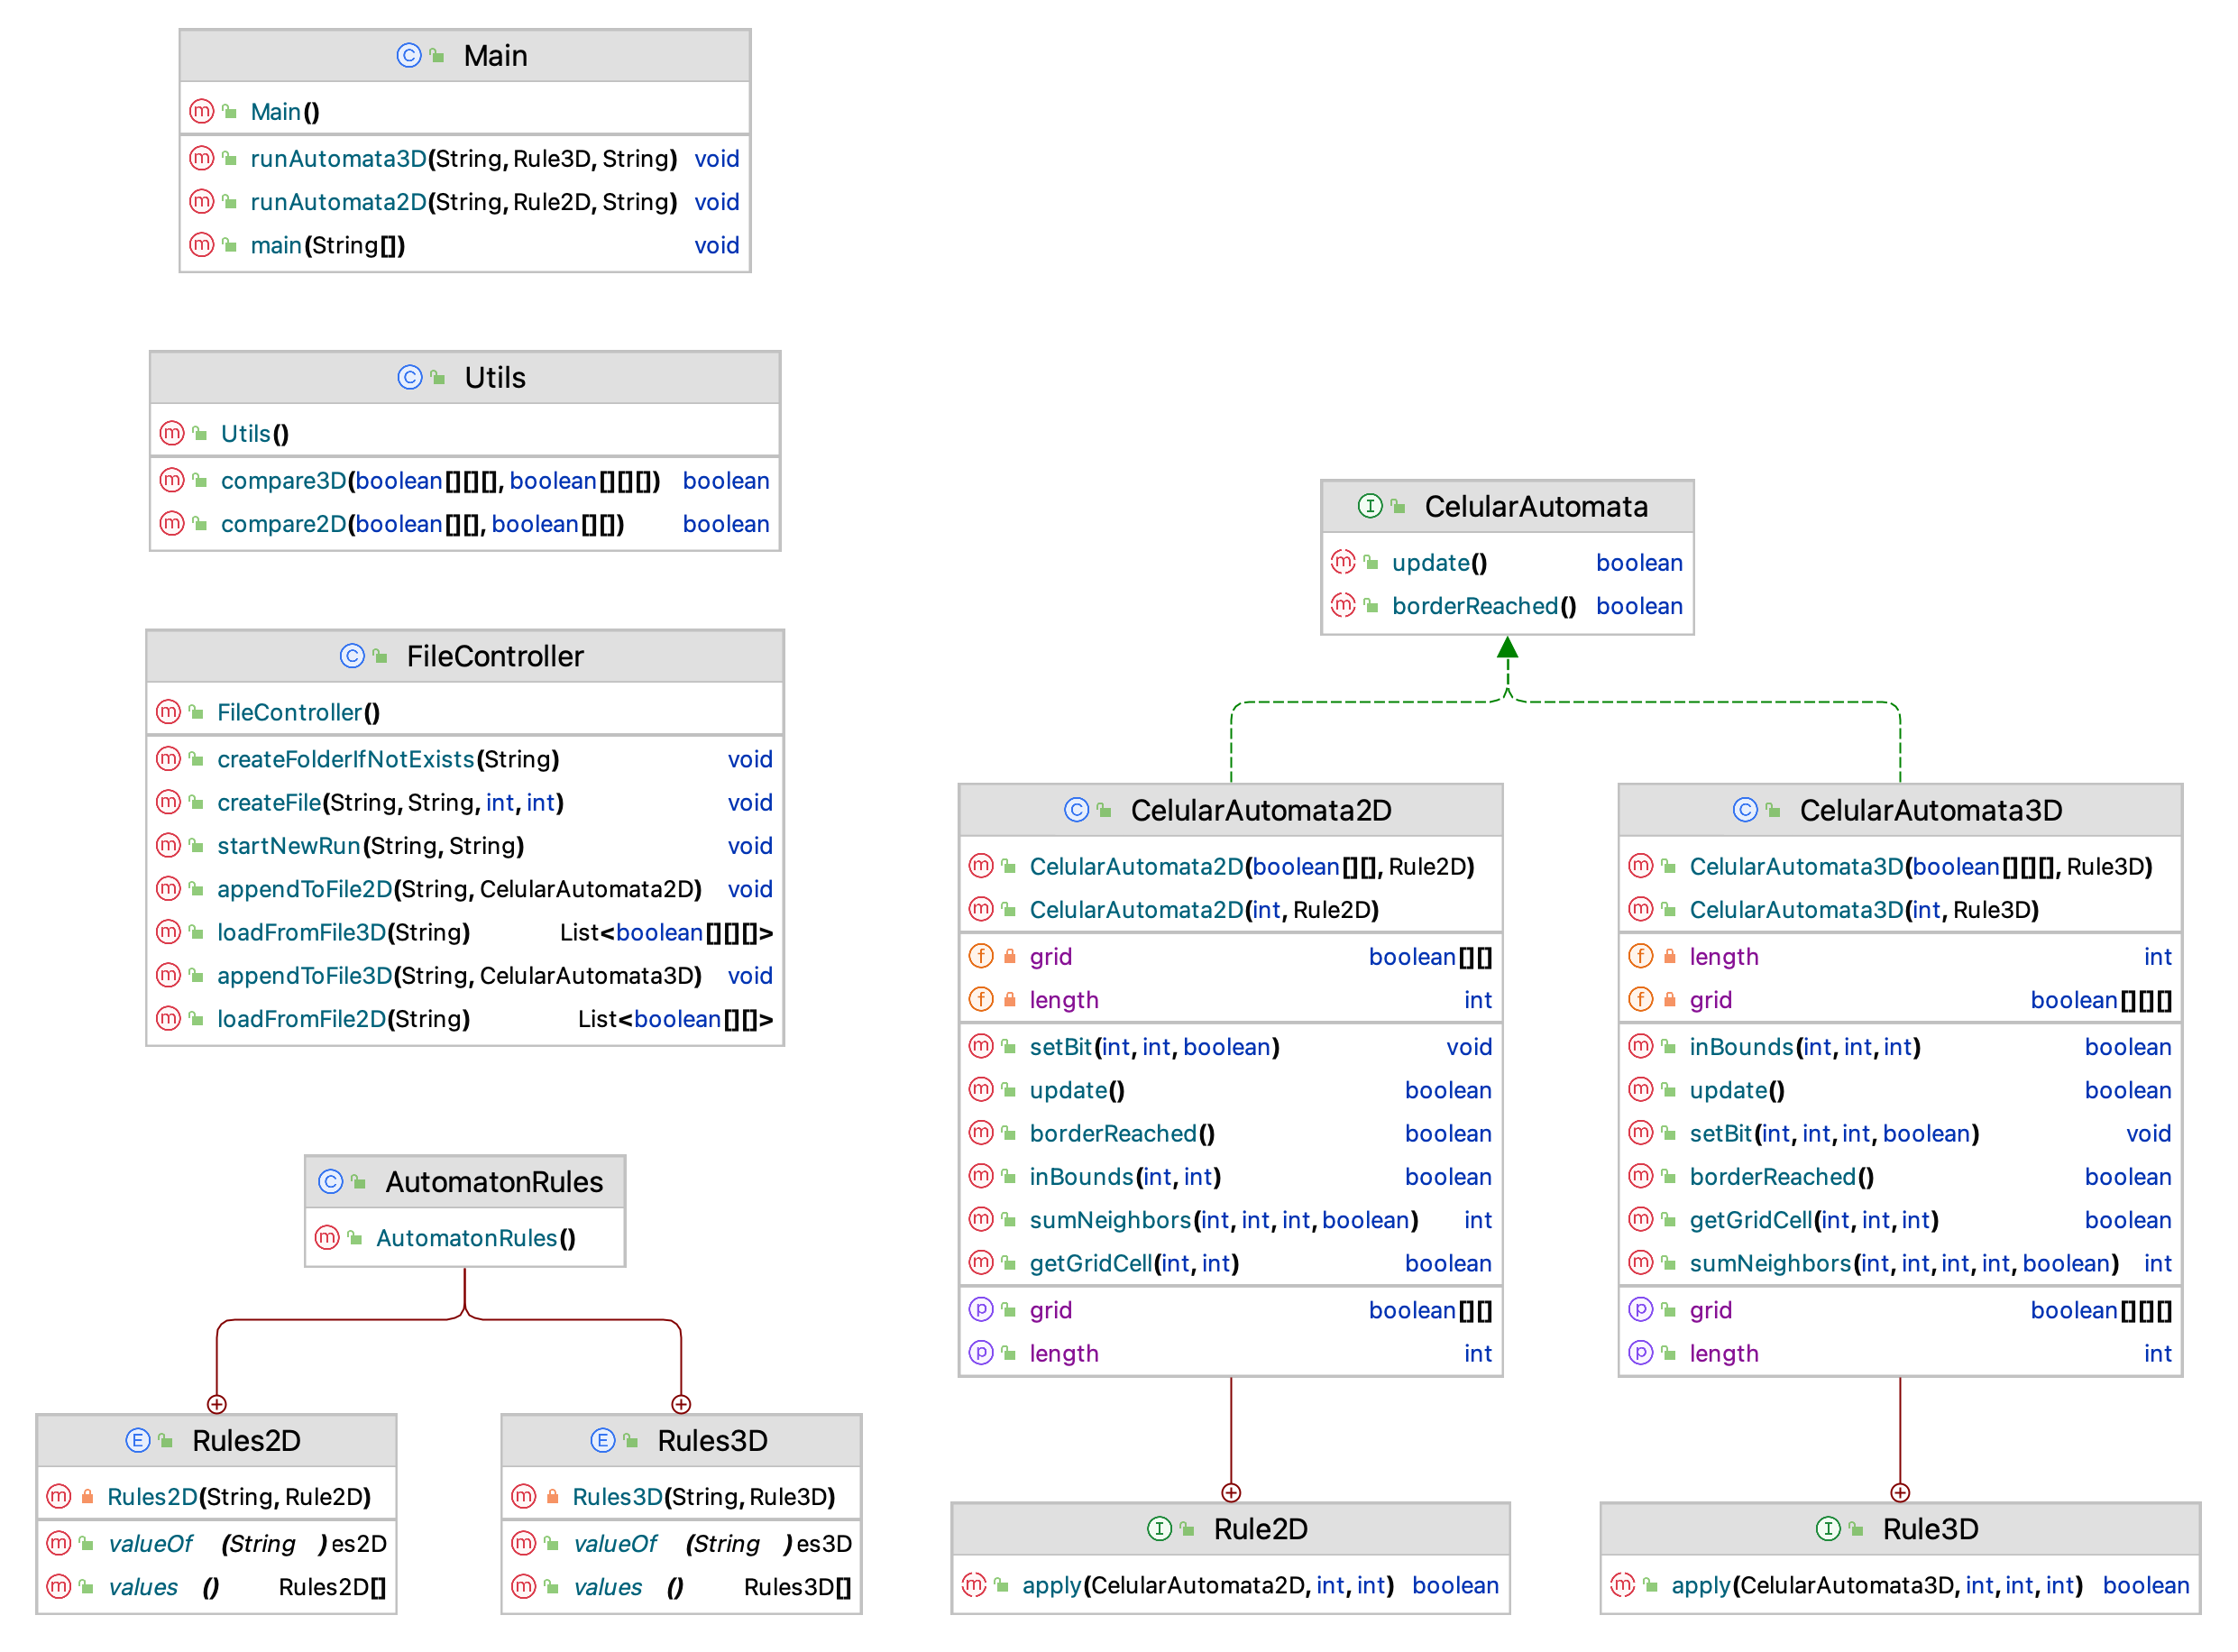
\includegraphics[width=1\textwidth]{Images/uml_light}
    \caption{Diagrama de clases}
    \label{fig:uml}
\end{figure}

\subsection{Clase \texttt{Main}}
\label{subsec:main}
En \texttt{Main} se definen la cantidad de celdas vivas iniciales para cada simulación, la cantidad de generaciones a simular y el tipo de autómata celular a utilizar.
Además, se inicializa el autómata celular y se ejecuta la simulación.

Trabaja con matrices de booleanos para representar el estado de las celdas en cada generación.

Estas se leen de archivos de texto de nombre \texttt{init\{2|3\}d\_[cantidad de celdas iniciales].txt} ubicados en la carpeta \texttt{input}.
El resultado de la simulación se guarda en distintos archivos de texto en la carpeta \texttt{output}, dentro de subcarpetas con el nombre del tipo de autómata celular.

%\subsection{Clase \texttt{FileController}}
%\label{subsec:filecontroller}
%\texttt{FileController} se encarga de leer y escribir carpetas y archivos de texto.
%
%\subsubsection{Lectura}
%\label{subsubsec:lectura}
%Es responsable de obtener los estados iniciales de los autómatas, a partir de los archivos de texto mencionados en la sección anterior.
%El formato de los archivos es el siguiente:
%\begin{itemize}
%    \item La primera línea contiene un entero que representa el lado la grilla cuadrada.
%    \item La segunda linea contiene un entero que indica el lado del cuadrado interno que contiene las celdas vivas iniciales.
%    \item Las siguientes líneas contienen cada una, una matriz de booleanos, donde \texttt{0} representa una celda muerta y \texttt{1} una celda viva.
%    \item En total hay 10 matrices, para tener 10 variantes de una misma cantidad de celulas iniciales vivas.
%\end{itemize}
%
%\subsubsection{Escritura}
%\label{subsubsec:escritura}
%Es responsable de escribir cada uno de los estados de las celdas en cada generación en archivos de texto.
%El formato de los archivos es el siguiente:
%\begin{itemize}
%    \item La primera línea contiene un entero que representa el lado la grilla cuadrada.
%    \item La segunda linea contiene un entero que indica el lado del cuadrado interno que contiene las celdas vivas iniciales.
%    \item La tercera linea se deja en blanco.
%    \item Las siguientes líneas contienen cada una, una matriz de booleanos, donde \texttt{0} representa una celda muerta y \texttt{1} una celda viva.
%    \item Cada linea representa una generación de la simulación.
%\end{itemize}

\subsection{Clases \texttt{CelularAutomata2D} y \texttt{CelularAutomata3D}}
\label{subsec:celularautomata}
Estas clases se encargan de simular el autómata celular en 2 y 3 dimensiones, respectivamente.

Ofrecen métodos para evolucionar el sistema en una generación y para obtener la cantidad de vecinos vivos de una celda en particular, usando distancia de Moore y Von Neumann.

También permiten saber si una celda está viva o muerta en una generación dada, si una posición se encuentra dentro de los límites de la grilla y si se alcanzó la condición de corte de contacto con el borde.

\subsection{Clase \texttt{AutomatonRules}}
\label{subsec:automatonrules}
\texttt{AutomatonRules} define las reglas de los autómatas celulares implementados.
Se implementa a partir de dos enums, \texttt{Rules2D} y \texttt{Rules3D}, que contienen las reglas de los autómatas celulares de dos y tres dimensiones, respectivamente.

Cada regla tiene asociada una función que determina si una celda debe estar viva o muerta en la siguiente generación, además de un nombre corto para identificar la regla.